\documentclass[journal]{IEEEtran}

\hyphenation{op-tical net-works semi-conduc-tor}
\usepackage{times}
\usepackage{epsfig}
\usepackage{graphicx}
\usepackage{amsmath}
\usepackage{amssymb}

% Include other packages here, before hyperref.
\usepackage[inline]{enumitem}
\usepackage{multirow}
\usepackage[style=ieee]{biblatex}
\bibliography{../presentation/depth}

% If you comment hyperref and then uncomment it, you should delete
% egpaper.aux before re-running latex.  (Or just hit 'q' on the first latex
% run, let it finish, and you should be clear).
\usepackage[breaklinks=true,bookmarks=true]{hyperref}

\begin{document}

	%
	% paper title
	% Titles are generally capitalized except for words such as a, an, and, as,
	% at, but, by, for, in, nor, of, on, or, the, to and up, which are usually
	% not capitalized unless they are the first or last word of the title.
	% Linebreaks \\ can be used within to get better formatting as desired.
	% Do not put math or special symbols in the title.
	\title{Images Classification with Estimated Depth Map}
	%
	%
	% author names and IEEE memberships
	% note positions of commas and nonbreaking spaces ( ~ ) LaTeX will not break
	% a structure at a ~ so this keeps an author's name from being broken across
	% two lines.
	% use \thanks{} to gain access to the first footnote area
	% a separate \thanks must be used for each paragraph as LaTeX2e's \thanks
	% was not built to handle multiple paragraphs
	%
	
	\author{Yihui~He% <-this % stops a space
		\thanks{Y. He was with the Department
			of Computer Science, Xi'an Jiaotong University, Xi'an,
			710049 China e-mail: yihuihe@foxmail.com (see http://yihui-he.github.io).}% <-this % stops a space
		}
	
	% note the % following the last \IEEEmembership and also \thanks - 
	% these prevent an unwanted space from occurring between the last author name
	% and the end of the author line. i.e., if you had this:
	% 
	% \author{....lastname \thanks{...} \thanks{...} }
	%                     ^------------^------------^----Do not want these spaces!
	%
	% a space would be appended to the last name and could cause every name on that
	% line to be shifted left slightly. This is one of those "LaTeX things". For
	% instance, "\textbf{A} \textbf{B}" will typeset as "A B" not "AB". To get
	% "AB" then you have to do: "\textbf{A}\textbf{B}"
	% \thanks is no different in this regard, so shield the last } of each \thanks
	% that ends a line with a % and do not let a space in before the next \thanks.
	% Spaces after \IEEEmembership other than the last one are OK (and needed) as
	% you are supposed to have spaces between the names. For what it is worth,
	% this is a minor point as most people would not even notice if the said evil
	% space somehow managed to creep in.
	
	
	
	% The paper headers
	\markboth{Journal of \LaTeX\ Class Files,~Vol.~14, No.~8, April~2017}%
	{He \MakeLowercase{\textit{et al.}}: Images Classification with Estimated Depth Map}
	% The only time the second header will appear is for the odd numbered pages
	% after the title page when using the twoside option.
	% 
	% *** Note that you probably will NOT want to include the author's ***
	% *** name in the headers of peer review papers.                   ***
	% You can use \ifCLASSOPTIONpeerreview for conditional compilation here if
	% you desire.
	
	
	
	
	% If you want to put a publisher's ID mark on the page you can do it like
	% this:
	%\IEEEpubid{0000--0000/00\$00.00~\copyright~2015 IEEE}
	% Remember, if you use this you must call \IEEEpubidadjcol in the second
	% column for its text to clear the IEEEpubid mark.
	
	
	
	% use for special paper notices
	%\IEEEspecialpapernotice{(Invited Paper)}
	
	
	
	
	% make the title area
	\maketitle
	
	% As a general rule, do not put math, special symbols or citations
	% in the abstract or keywords.
	\begin{abstract}
We consider the problem of doing image classification using estimated depth 
information. This problem clearly falls into the domain of transfer learning, since we are using a model trained on a set of depth images in order to generate depth maps (additional features) for use in another classification problem using another disjoint set of images. It is a challenging task as no direct depth information is 
provided. Previous related research efforts have been focused on image classification tasks using
RGB images and depth image estimation but none have attempted to use depth image estimations in order to aid image classification over RGB images. Therefore, in this paper we present a way of 
transferring domain knowledge on depth estimation to a seperate image classification task over a disjoint set of training, validation and test data. 
To our knowledge, we are the first to bridge gap between image classification and depth estimation.

Specifically, we attempt to implement the recent work by \cite{liu2015deep}, build a RGBD dataset and do image classification 
on the RGBD dataset we built and then compare the performance of both a simple feedforward neural network and a multi-layer convolutional neural network of the RGBD dataset compared to the RGB dataset.
Our project code, models, and example results are available on github \cite{he2016depth}.
	\end{abstract}
	
	% Note that keywords are not normally used for peerreview papers.
	\begin{IEEEkeywords}
		convolutional neural networks, depth estimation, image recognition.
	\end{IEEEkeywords}
	
	
	
	
	
	
	% For peer review papers, you can put extra information on the cover
	% page as needed:
	% \ifCLASSOPTIONpeerreview
	% \begin{center} \bfseries EDICS Category: 3-BBND \end{center}
	% \fi
	%
	% For peerreview papers, this IEEEtran command inserts a page break and
	% creates the second title. It will be ignored for other modes.
	\IEEEpeerreviewmaketitle
	
	
	
	\section{Introduction}
	% The very first letter is a 2 line initial drop letter followed
	% by the rest of the first word in caps.
	% 
	% form to use if the first word consists of a single letter:
	% \IEEEPARstart{A}{demo} file is ....
	% 
	% form to use if you need the single drop letter followed by
	% normal text (unknown if ever used by the IEEE):
	% \IEEEPARstart{A}{}demo file is ....
	% 
	% Some journals put the first two words in caps:
	% \IEEEPARstart{T}{his demo} file is ....
	% 
	% Here we have the typical use of a "T" for an initial drop letter
	% and "HIS" in caps to complete the first word.
	\IEEEPARstart{E}{stimating} depths from a single monocular image depicting 
	general scenes is a fundamental problem in computer vision, 
	which has widespread applications in scene-understanding, 
	3D modeling, robotics, and other challenging problems.
	It is a notorious example of an ill-posed problem, 
	as one captured image may correspond to numerous real world scenes \cite{eigen2014depth}. 
	it remains a challenging task for computer vision algorithms as no reliable cues can be exploited,
	such as temporal information, stereo correspondences.
	Previous research involving depth-maps usually involve
	geometric \cite{hedau2010thinking,gupta2010estimating,gupta2010blocks}, convolutional \cite{liu2015deep}, and semantic \cite{ladicky2014pulling} techniques.
	Nevertheless, none of these works tried to perform image classification using depth maps as training data.
	Different from previous efforts, 
	we propose to utilize depth maps in a image classification task.
	While extensively studied in semantic labeling and accuracy improvement,
	depth map regression has been less explored in its application to classification problems. Theoretically, one can imagine that a neural-network that is deep enough would generate it's own depth-map (or at least simulate depth-map-like features).
	
	Recently, the efficacy and power of the deep
	convolutional neural network (CNN) has been made accessible \cite{krizhevsky2012imagenet,Simonyan2014}. 
	With a CNN, we are able to perform depth estimation on a single image \cite{liu2015deep}.
	However, most classification tasks still perform on RGB images \cite{He2015,he2016identity,xie2016aggregated}.
	With only RGB images, CNN features have been setting new records for a wide variety of vision applications \cite{razavian2014cnn,fasterrcnn,long2015fully}.
	Despite all the successes in depth estimation and image classification,
	the deep CNN has been not yet been used for learning on RGBD images, since RGBD datasets are not as widely-used as RGB datasets .
	To our knowledge, we are the first to bridge gap between depth estimation and image classification.
	
	To sum up, we highlight the main contributions of this work as follows:
	\begin{itemize}
		\vspace{-.12cm} \item 
		We implemented a deep convolutional neural field in order to solve the depth estimation problem and obtained similar results to the implementation used in the paper.
		\vspace{-.12cm} \item
		We created the first RGBD image dataset for CIFAR-10.
		\vspace{-.12cm} \item 
		We define a new metric for ill-posed depth prediction problem.
		\vspace{-.12cm} \item 
		We prove that depth channel has a better feature representation than R,G,B channels,
		and show that training on RGBD images can somehow improve accuracy.
	\end{itemize}
	
%	\hfill mds
	
	\hfill April 21, 2017
	
	
	% An example of a floating figure using the graphicx package.
	% Note that \label must occur AFTER (or within) \caption.
	% For figures, \caption should occur after the \includegraphics.
	% Note that IEEEtran v1.7 and later has special internal code that
	% is designed to preserve the operation of \label within \caption
	% even when the captionsoff option is in effect. However, because
	% of issues like this, it may be the safest practice to put all your
	% \label just after \caption rather than within \caption{}.
	%
	% Reminder: the "draftcls" or "draftclsnofoot", not "draft", class
	% option should be used if it is desired that the figures are to be
	% displayed while in draft mode.
	%
	%\begin{figure}[!t]
	%\centering
	%\includegraphics[width=2.5in]{myfigure}
	% where an .eps filename suffix will be assumed under latex, 
	% and a .pdf suffix will be assumed for pdflatex; or what has been declared
	% via \DeclareGraphicsExtensions.
	%\caption{Simulation results for the network.}
	%\label{fig_sim}
	%\end{figure}
	
	% Note that the IEEE typically puts floats only at the top, even when this
	% results in a large percentage of a column being occupied by floats.
	
	
	% An example of a double column floating figure using two subfigures.
	% (The subfig.sty package must be loaded for this to work.)
	% The subfigure \label commands are set within each subfloat command,
	% and the \label for the overall figure must come after \caption.
	% \hfil is used as a separator to get equal spacing.
	% Watch out that the combined width of all the subfigures on a 
	% line do not exceed the text width or a line break will occur.
	%
	%\begin{figure*}[!t]
	%\centering
	%\subfloat[Case I]{\includegraphics[width=2.5in]{box}%
	%\label{fig_first_case}}
	%\hfil
	%\subfloat[Case II]{\includegraphics[width=2.5in]{box}%
	%\label{fig_second_case}}
	%\caption{Simulation results for the network.}
	%\label{fig_sim}
	%\end{figure*}
	%
	% Note that often IEEE papers with subfigures do not employ subfigure
	% captions (using the optional argument to \subfloat[]), but instead will
	% reference/describe all of them (a), (b), etc., within the main caption.
	% Be aware that for subfig.sty to generate the (a), (b), etc., subfigure
	% labels, the optional argument to \subfloat must be present. If a
	% subcaption is not desired, just leave its contents blank,
	% e.g., \subfloat[].
	
	
	% An example of a floating table. Note that, for IEEE style tables, the
	% \caption command should come BEFORE the table and, given that table
	% captions serve much like titles, are usually capitalized except for words
	% such as a, an, and, as, at, but, by, for, in, nor, of, on, or, the, to
	% and up, which are usually not capitalized unless they are the first or
	% last word of the caption. Table text will default to \footnotesize as
	% the IEEE normally uses this smaller font for tables.
	% The \label must come after \caption as always.
	%
	%\begin{table}[!t]
	%% increase table row spacing, adjust to taste
	%\renewcommand{\arraystretch}{1.3}
	% if using array.sty, it might be a good idea to tweak the value of
	% \extrarowheight as needed to properly center the text within the cells
	%\caption{An Example of a Table}
	%\label{table_example}
	%\centering
	%% Some packages, such as MDW tools, offer better commands for making tables
	%% than the plain LaTeX2e tabular which is used here.
	%\begin{tabular}{|c||c|}
	%\hline
	%One & Two\\
	%\hline
	%Three & Four\\
	%\hline
	%\end{tabular}
	%\end{table}
	
	
	% Note that the IEEE does not put floats in the very first column
	% - or typically anywhere on the first page for that matter. Also,
	% in-text middle ("here") positioning is typically not used, but it
	% is allowed and encouraged for Computer Society conferences (but
	% not Computer Society journals). Most IEEE journals/conferences use
	% top floats exclusively. 
	% Note that, LaTeX2e, unlike IEEE journals/conferences, places
	% footnotes above bottom floats. This can be corrected via the
	% \fnbelowfloat command of the stfloats package.
	
\section{Related Work}
Convolutional networks have been applied with great success for object 
classification and detection. CNNs have recently been applied to a variety 
of other tasks, like depth estimation. Depth estimation from single image is 
well addressed by \cite{liu2015deep} and \cite{eigen2015predicting}. They both agree that depth estimation 
is an ill-posed problem, since there's no real ground truth depth map. By 
contrast, we define transfer learning accuracy metric for depth estimation 
model. It becomes easier to compare performance of different depth estimation 
model.

Depth map has been successfully applied to some problems. based on depth 
information, performance improvement on semantic 
labeling \cite{eigen2015predicting} has been seen. however, depth maps have not
been combined with an image classification task. To our knowledge, we are the first to 
bridge gap between depth estimation and image classification.

Our work builds upon state-of-the-art depth estimation model \cite{liu2015deep}
which is a two loss neural network. We used this model in order to build the RGBD dataset, and investigate the
quality the depth maps. Moreover, we improved 
accuracy of image classification task with depth map data.

%-------------------------------------------------------------------------
\section{Deep Convolutional Neural Field}
We present the details of deep convolutional neural field model we used for 
depth estimation in this section. 
\subsection{Theory and Architecture}
The goal here is to infer the depth of each pixel in a single image depicting 
general scenes. we make the common assumption that an image is composed of small 
homogeneous regions (superpixels). 
Let $x$ be an image and $y=[y_1,...,y_n]^T\in R^n$ be a vector of continuous 
depth values corresponding to all n superpixels in x. We model the conditional 
probability as softmax:
\begin{equation}
Pr(y|x)=\frac{exp(-E(y,x))}{\sum_i 
	exp(E(y_i,x))}
\end{equation}
where $E$ is energy function.
To predict the depths of a new image, we solve the maximum a posteriori (MAP) 
inference problem: 
\begin{equation}
\label{eq:inference}
y^{\star}=\arg\max\limits_y Pr(y|x). 
\end{equation}
We formulate the energy function as a 
typical combination of unary potentials U and pairwise potentials V over the 
nodes (superpixels) N and edges S of the image x:
\begin{equation}\label{eq:energy}
E(y, x) = \sum_{p \in {\cal N} } U(y_{p}, x) 
+ \sum_{(p,q) \in {\cal S}} V(y_{p}, y_{q}, x).
\end{equation}
The unary term U aims to regress the depth value from a single superpixel. The 
pairwise term V encourages neighboring superpixels with similar appearances 
to take similar depths. We aim to jointly learn U and V in a unified CNN 
framework.
In Figure~\ref{fig:arch} , we show a sketch of our deep convolutional
neural field model for depth estimation. As we can see, the whole network is 
composed of a unary part, a pairwise part and a CRF loss layer.
\begin{figure*}
	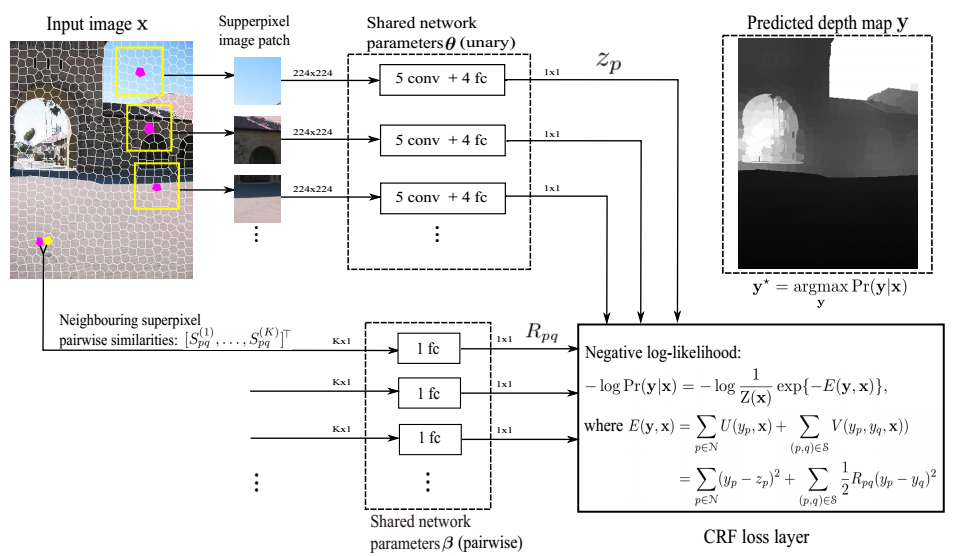
\includegraphics[width=.9\linewidth]{arch.png}
	\caption{Deep Convolutional Neural Field model}
	\label{fig:arch}
\end{figure*}

For an input image, which has been segmented into n superpixels, we 
consider image patches centered around each superpixel centroid. The unary part 
then takes all the image patches as input and feed each of them to a CNN and 
output an n-dimensional vector containing regressed depth values of the n 
superpixels. The network for the unary part is composed of 5 convolutional and 
4 fully-connected layers with details in Figure~\ref{fig:unary}. 
\begin{figure*}
	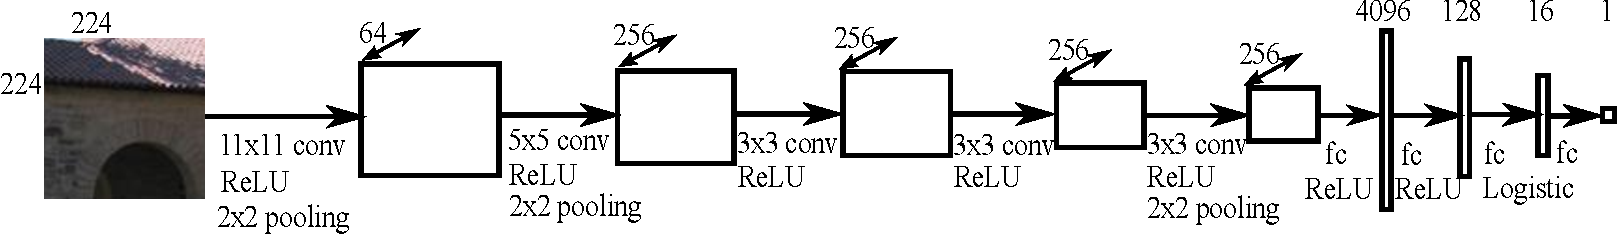
\includegraphics[width=\linewidth]{../presentation/fig/cnn_unary.pdf}
	\caption{unary part of Deep Convolutional Neural Field model}
	\label{fig:unary}
\end{figure*}

Kindly note that the CNN parameters are shared across all the superpixels. 
The pairwise part takes similarity vectors (each with K components) of all 
neighboring superpixel pairs as input and feed each of them to a 
fully-connected layer (parameters are shared among different pairs), then output 
a vector containing all the 1-dimensional similarities for each of the neighboring superpixel pair. The CRF loss layer takes as input the outputs from 
the unary and the pairwise parts to minimize the negative log-likelihood.
\subsubsection{Unary part}
The unary potential is constructed from the output of a CNN by considering the least square loss:
\begin{equation}\label{eq:unary}
U(y_{p}, x;\theta) = (y_p - \hat{y}_p (\theta))^2, \;\; \forall p=1,...,n.
\end{equation}
Here $\hat{y}_p$ is the regressed depth of the superpixel $p$ parametrized by 
the CNN parameters $\theta$. The network architecture for the unary part is 
depicted in Figure~\ref{fig:unary}. It is composed of 5 convolutional layers 
and 4 fully connected layers. The input image is first segmented into 
superpixels, then for each superpixel, we consider the image patch centered 
around its centroid. Each of the image patches is resized to 224×224 pixels and 
then fed to the convolutional neural network. Note that the convolutional and 
the fully-connected layers are shared across all the image patches of different 
superpixels.
\subsubsection{Pairwise part}
We construct the pairwise potential from 3 types of similarity observations: 
color difference, color histogram difference and texture 
disparity \cite{ojala1994performance}. Each of them enforces smoothness by 
exploiting consistency information of neighboring superpixels:
\begin{equation}
\label{eq:pairwise}
V(y_{p}, y_{q}, x; \beta) = \sum_{k=1}^K \beta_k S_{pq}^{(k)}(y_p - y_q)^2, 
\;\forall p,q=1,...,n.
\end{equation}
Here, $K=3$ in our case. $S_{pq}$is similarity of two neighbor superpixels $p$ 
and $q$. $\beta$ is trainable parameters, so we can let CNN decide which 
similarity is more important. 

\subsection{Implementation Details}
We implement the network training on Make3D \cite{saxena2005learning} dataset 
with Tensorflow \cite{tensorflow2015-whitepaper}. Make3D dataset contains 
more outdoor scenes, which makes it easier for us to transfer learning onto the
CIFAR10 dataset. During each SGD iteration, 
around ∼ 700 superpixel image patches are processed. Our implementation differs from the 
original implementation \cite{liu2015deep}, Since we have enough memory, we feed 
700 superpixel image patches into memory at once. Other parts of implementation are similar to how they are described in the paper.

During implementation, we initialize the first 6 layers of the unary part in 
Figure~\ref{fig:unary} using a CNN model trained on the ImageNet 
from \cite{chatfield2014return}. First, we do not back propagate through the 
previous 6 layers by keeping them fixed and train the rest of the network
with momentum 0.9, learning rate 0.0001, and weight decay 
0.0005. Then we train the whole network with the same momentum and weight decay.

\subsection{Experiment}
We measure our performance on Make3D dataset and compare our result with \cite{liu2015deep} as a sanity check. 

The Make3D dataset contains 534 images depicting outdoor scenes. As pointed out 
in \cite{liu2014discrete}, this dataset is with limitations: the maximum value 
of depths is 81m with far objects are all mapped to the one distance of 81 
me- ters. As a remedy, two criteria are used to report the prediction error (C1) 
Errors are calculated only in the regions with the ground-truth depth less 
than 70 meters; (C2) Errors are calculated over the entire image. We follow this 
protocol.
Performance is shown in Table~\ref{tab:sanity}. 
You can see that
our model achieve pretty close result, which allows us do further research on depth map.
\begin{table} \center
	\resizebox{\linewidth}{!} {
		\begin{tabular}{ | l |  c  c  c | c  c  c |}
			\hline 
			\multirow{3}{*}{{{Method}}} &\multicolumn{3}{c|}{Error(C1)} 
			&\multicolumn{3}{c|}{Error(C2)} \\
			&\multicolumn{3}{c|}{(lower is better)} &\multicolumn{3}{c|}{(lower is better)} 
			\\
			\cline{2-7}
			&rel &log10 &rms &rel &log10 &rms  \\
			\hline
			%
			%
			Our implementation &0.335&0.137&9.49&0.338&0.134&14.60 \\
			Original paper    &\textbf{0.314}&\textbf{0.119}  &\textbf{8.60}  
			&\textbf{0.307} 	 &\textbf{0.125}	 &\textbf{12.89} \\
			\hline
		\end{tabular}
	}
	\caption{Sanity check (\textbf{Bold} is better)}
	\label{tab:sanity}
\end{table}

In Figure~\ref{fig:depthest} we also show depth maps our model learned.
\begin{figure}
	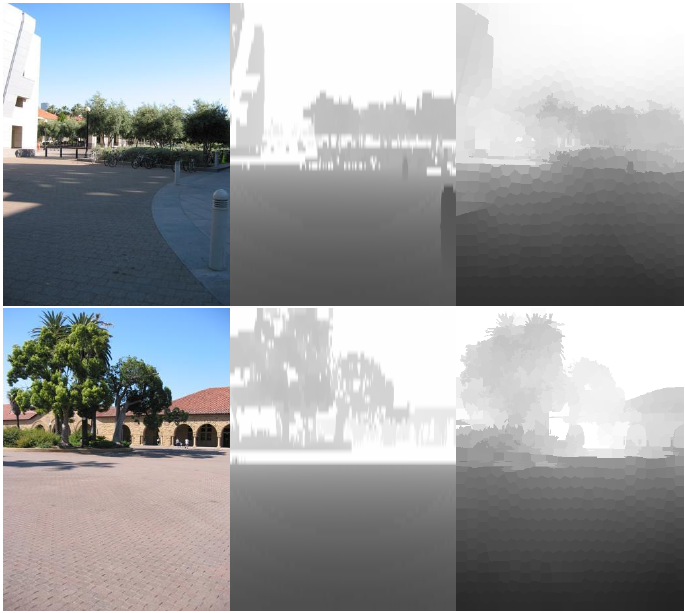
\includegraphics[width=\linewidth]{../learntd.png}
	\caption{original image, ground truth, depth estimation (from left to right)}
	\label{fig:depthest}
\end{figure}

%-------------------------------------------------------------------------
\section{RGBD Image for Classification}
Recent depth image research works mainly focus on depth-estimation \cite{liu2015deep} 
and segmentation with depth image \cite{eigen2015predicting}.
And we\rq{}ve witnessed significant improvement on depth estimation accuracy in these years. 
However, most image classification tasks nowadays are still performed on RGB images.
So we want to transfer depth knowledge learned by depth estimation model into our image-classification model.
In this section, 
we first built a RGBD dataset for CIFAR-10 \cite{krizhevsky2009learning}, 
based on a trained deep convolutional neural field model in the previous section. 
To investigate the effect of the depth channel on image classification task, 
we design two experiments (one with a simple feedforward NN and one with a CNN) 
Finally, we propose a new metric for depth estimation performance measurement.

\subsection{Build RGBD CIFAR10 Dataset}
Since the Deep Convolutional Neural Field model accepts images that are 
much larger that CIFAR-10 tiny images (32x32), we build RGBD dataset as follow:
\begin{enumerate}
	\item resize CIFAR10 tiny image (32x32x3) to normal size (400x400x3) in order to 
	feed in CNF.
	\item perform depth estimation on normal size image.
	\item downscale the output image (depth image, 400x400x1) back to tiny 
	image (32x32x1).
	\item combine RGB and D channels together as our RGBD image (32x32x4).
\end{enumerate}
Figure~\ref{fig:dataset} shows the transfer learning procedure.
\begin{figure}
	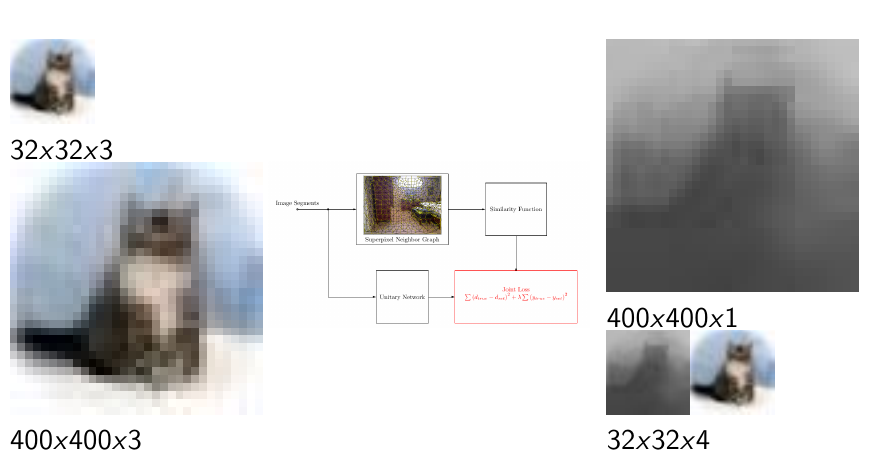
\includegraphics[width=\linewidth]{../dataset.png}
	\caption{Transer Learning: Build RGBD CIFAR10 dataset}
	\label{fig:dataset}
\end{figure}
Since there is no ground-truth depth image for CIFAR-10 dataset, we can\rq{}t directly 
measure the accuracy of our depth estimation attempts for these tiny images. 
However, we can infer this indirectly in two ways.
First we can look at these depth images
and make sure that most of them is reasonable.
Figure~\ref{fig:tiny} shows some depth maps.
Second, we can use the accuracy results of our two experiments as a new metric to 
quantify depth map quality.
\begin{figure}
	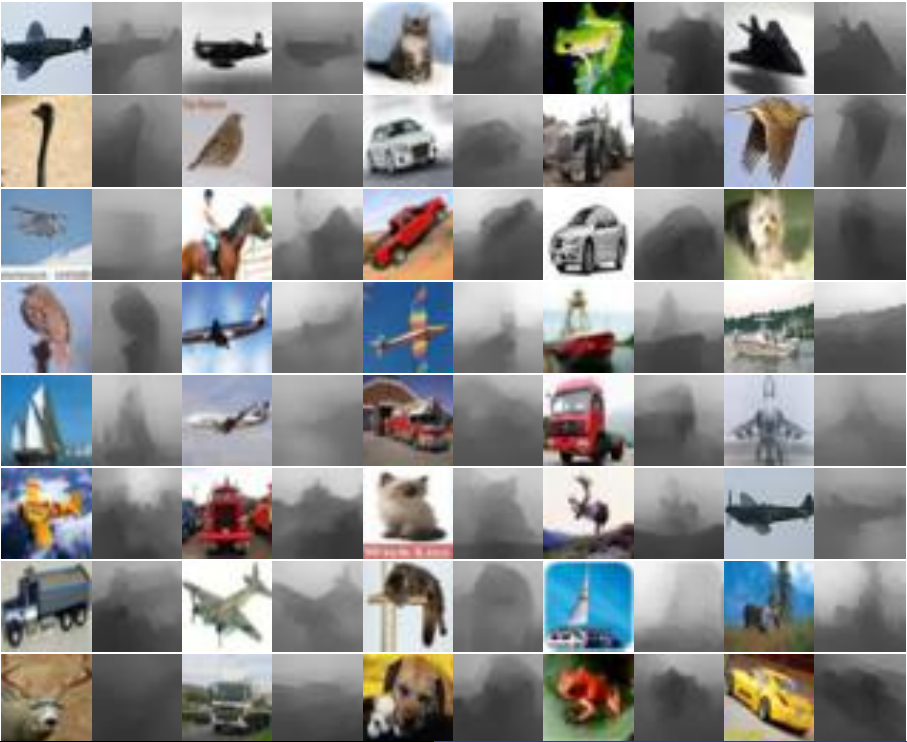
\includegraphics[width=\linewidth]{../tiny.png}
	\caption{Depth map estimated by deep convolutional neural field}
	\label{fig:tiny}
\end{figure}

\subsection{Classification Task on RGBD CIFAR10}
In order to make it easier to show effect of depth channel,
we employ a simple two layer neural network for classification task.
The architecture for learning on the RGBD dataset is shown in Figure~\ref{fig:tarch}. 
\begin{figure}
	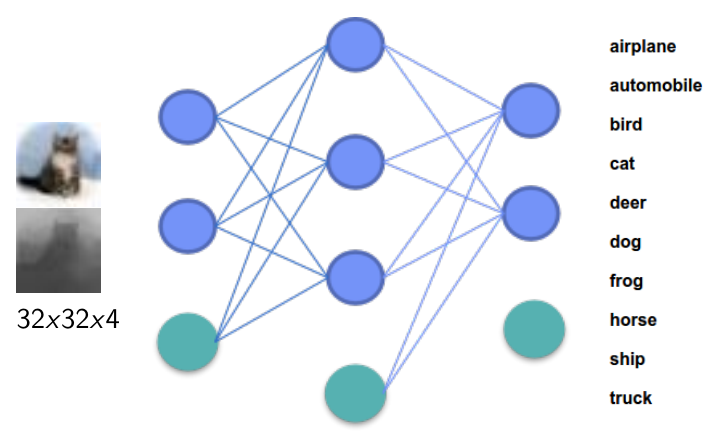
\includegraphics[width=\linewidth]{../Tarch.png}
	\caption{Learning on RGBD dataset}
	\label{fig:tarch}
\end{figure}
The number of neurons in the input layer depends on input.
If input is a single channel (R, G, B, D), we have 32x32 neurons.
The amount of hidden neurons is not determined. We perform fine tuning 
for each situation. The number of output neurons is always number of classes (10 classes
for CIFAR-10). Technical details of our architecture is shown in Table~\ref{tab:details}. 
Hyperparameters are not discussed here but will be fine tuned.
\begin{table}
	\begin{center}
		\begin{tabular}{|l|l|l|l|}
			\hline
			regularization&Activation&Update&batch\\
			\hline
			Dropout&ReLU&Momentum&128\\
			\hline
		\end{tabular}
	\end{center}
	\caption{Architecture details for classification task on our new RGBD dataset}
	\label{tab:details}
\end{table}


\subsection{Experiment}
We measure depth map quality in two ways. 
First, we train neural network on R, G, B, D channel as input respectively.
And compare their loss and accuracy. 
Second, we train neural network on RGB, RGBD respectively. 
And compare their loss and accuracy.

\subsubsection{R vs G vs B vs D}
We perform fine tuning on each channel. So that their performances are approximately optimal.
Figure~\ref{fig:channeltrain} shows training accuracy comparison through time. 
Figure~\ref{fig:channeltest} shows validation accuracy comparison through time. 
\begin{figure}
	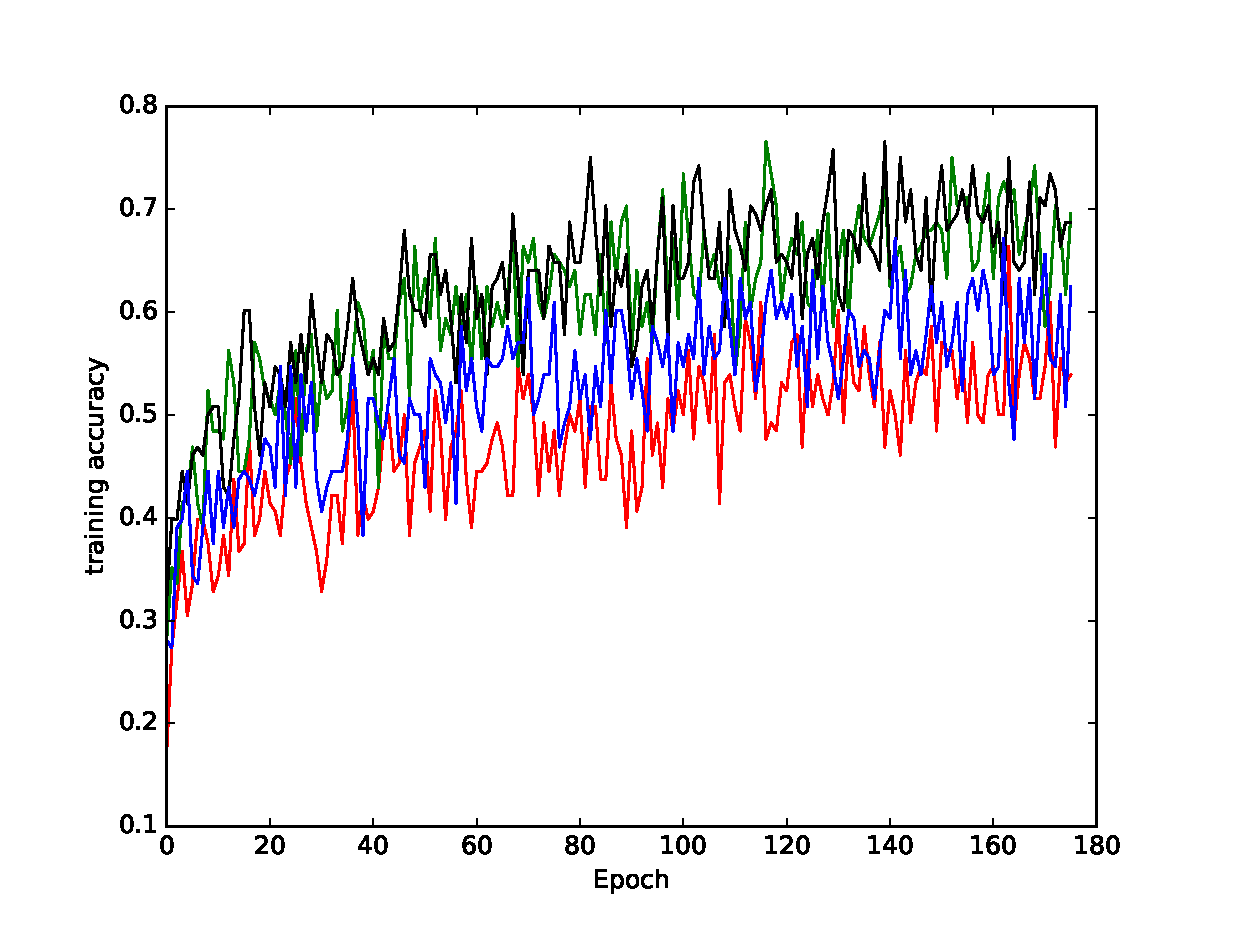
\includegraphics[width=\linewidth]{../presentation/train.eps}
	\caption{R vs G vs B vs D, training time}
	\label{fig:channeltrain}
\end{figure}
\begin{figure}
	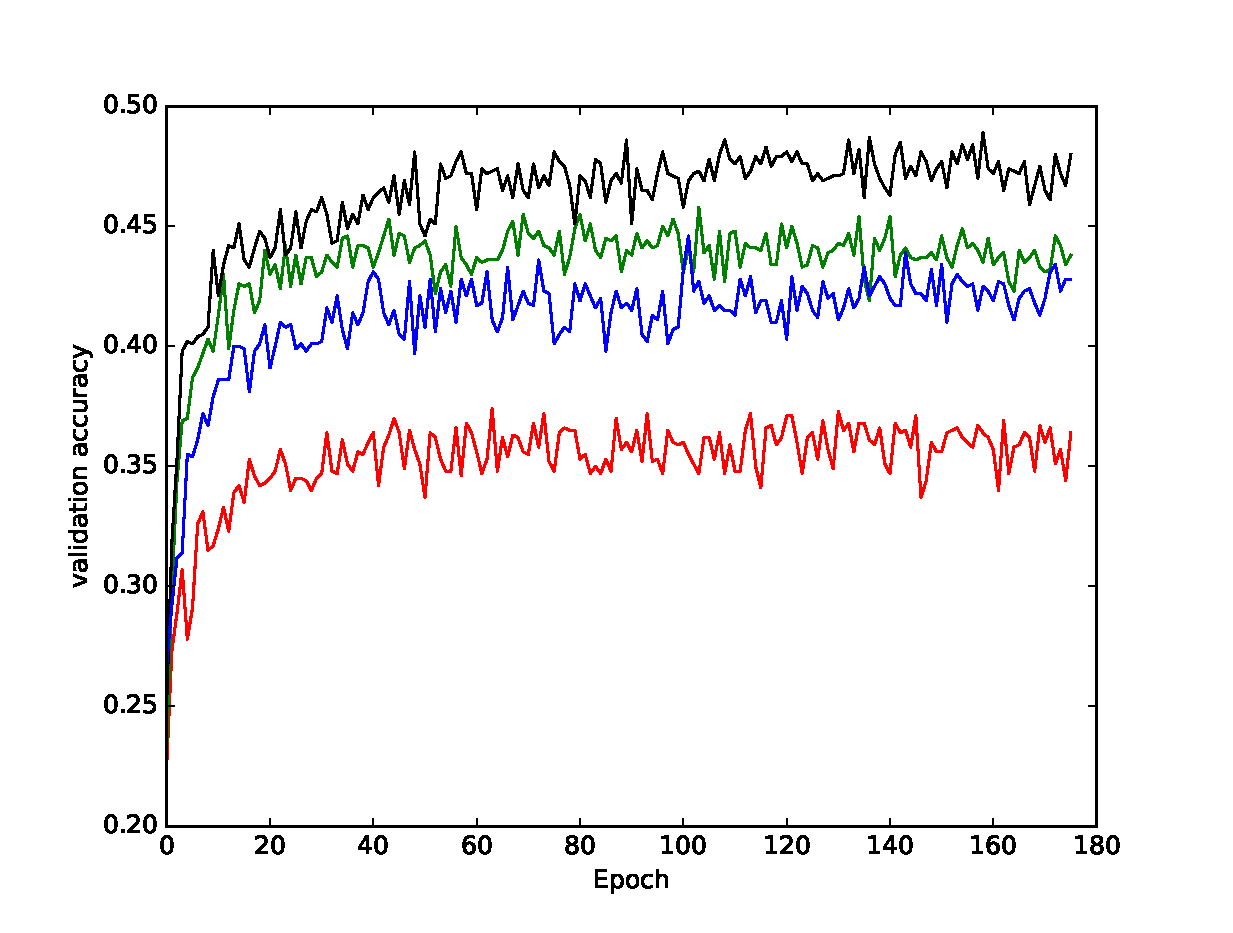
\includegraphics[width=\linewidth]{../presentation/test.eps}
	\caption{R vs G vs B vs D, testing time}
	\label{fig:channeltest}
\end{figure}

You can see that, at testing time, the depth channel outperforms R,G,B channels under the same architecture.
This implies that, depth channel has a better feature representation than R, G, B channels.

\subsubsection{RGB vs RGBD}
We perform fine tuning for both RGB and RGBD situations.
So that their performances are approximately optimal.
Figure~\ref{fig:mixtrain} Compares training accuracy  through time. 
Figure~\ref{fig:mixtest} Compares validation accuracy comparison through time. 
\begin{figure}
	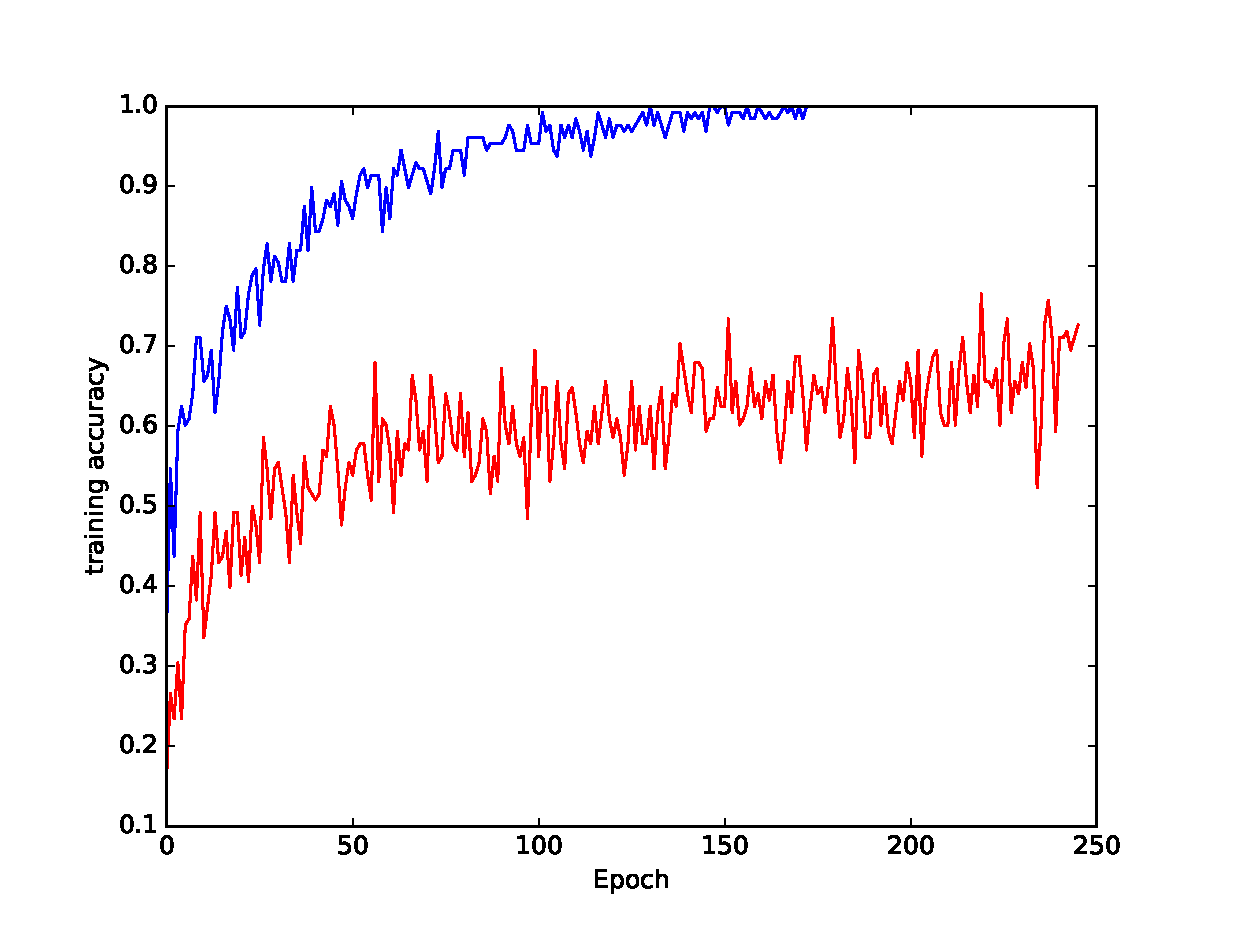
\includegraphics[width=\linewidth]{../presentation/together_train.eps}
	\caption{RGB vs RGBD, training time (RGBD:blue, RGB:red)}
	\label{fig:mixtrain}
\end{figure}
\begin{figure}
	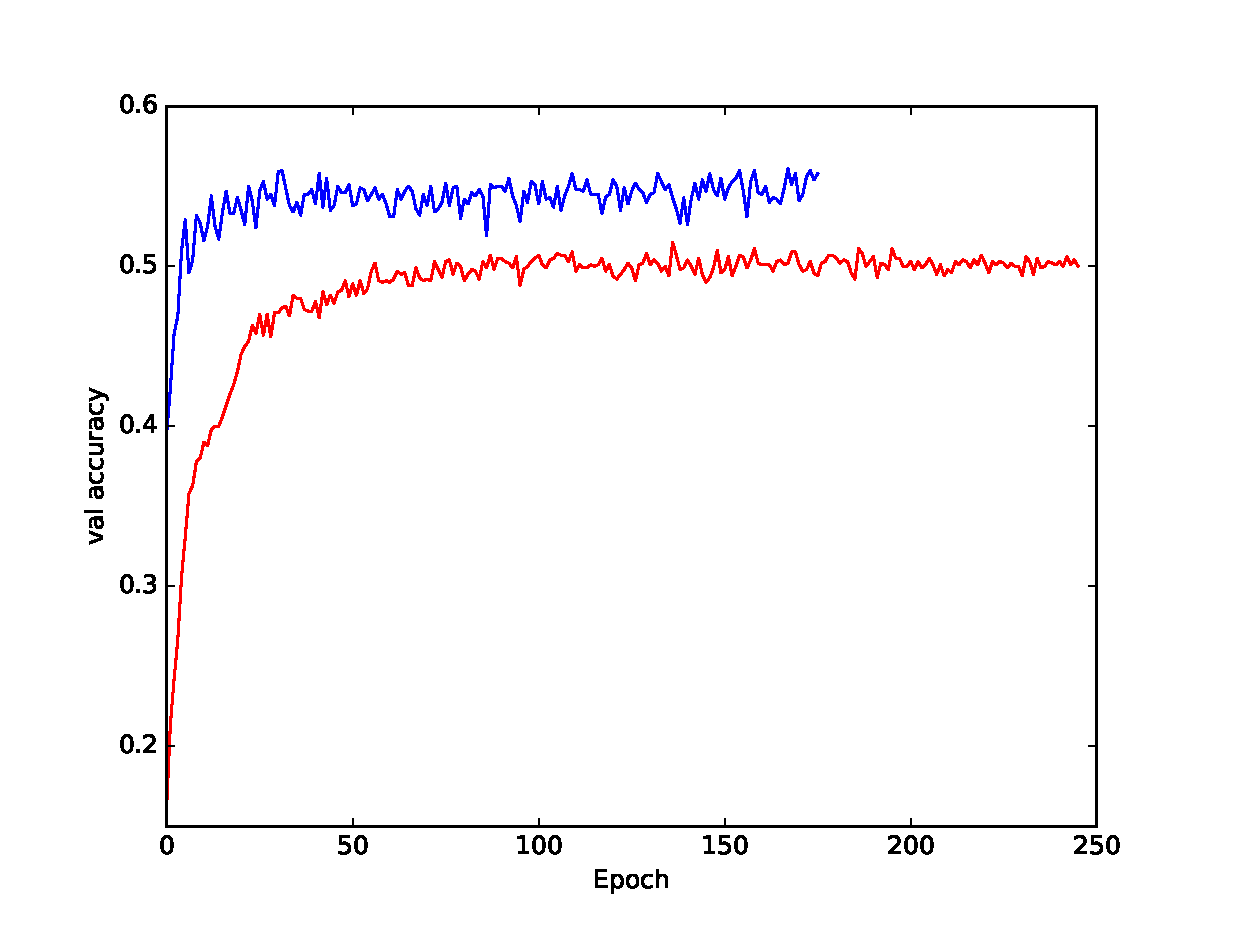
\includegraphics[width=\linewidth]{../presentation/together_test.eps}
	\caption{RGB vs RGBD, testing time (RGBD:blue, RGB:red)}
	\label{fig:mixtest}
\end{figure}

We get {\bf56\%} and {\bf52\%} validation accuracy with RGBD and RGB dataset respectively.
This can be seen as a sign that depth map brings extra knowledge
learned by deep convolutional neural field to our classification task.

You can also notice that, although RGBD dataset have more inputs and neurons,
it has a much higher converge rate than RGB dataset. 
It can be interpreted as a better feature representation brought by depth map.

\subsubsection{CNN Experimentation}
Our previous experiments using a 2-layer feedforward neural network yielded a performance increase of 4\% when comparing the accuracy of a NN trained on the RGB dataset to the NN trained on the RGBD dataset. These results did not satisfy us, as a simple feedforward neural network can show how good the features are presented to it, but not the optimal tool used for image classification. We want to see whether the estimated depth map truely bring in some new knowledges of depth, which can't be obtained just using RGB images. So we decided to test the performance of our CNN \cite{krizhevsky2012imagenet} over the CIFAR-10 RGB dataset and compare it to the performance achieved over our CIFAR-10 RGBD dataset. We achieved an accuracy of {\bf57.5\%} and {\bf53\%} using the RGBD and RGB datasets respectively. This performance gain of {\bf4.5\%} in accuracy between RGBD and RGB using the CNN is slightly better than the original accuracy gain {\bf4.0\%} using the 2-layer ANN.

Our convolutional neural network was composed of two convolutional layers (with subsequent max-pooling layers) followed by two fully-connected layers. 

Figure~\ref{fig:mixtest0},~\ref{fig:mixtest1},~\ref{fig:mixtest2} show results on convolutional neural network. We can see consistent results on 2-layers neural network and CNN.

\begin{figure}[!t]
	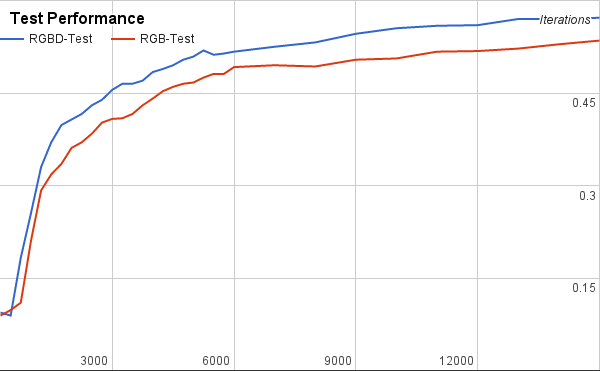
\includegraphics[width=\linewidth]{../presentation/test_conv.png}
	\caption{RGB vs RGBD Test CNN Accuracy, Iterations}
	\label{fig:mixtest0}
\end{figure}

\begin{figure}[!t]
	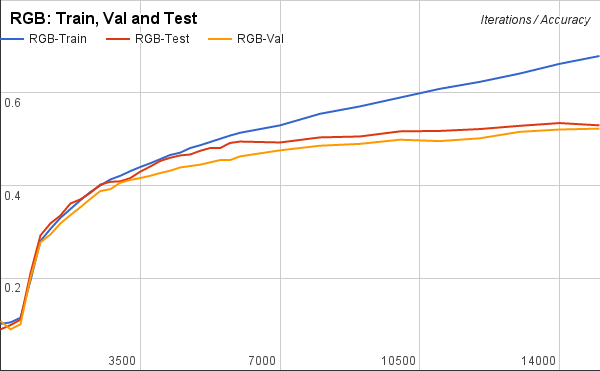
\includegraphics[width=\linewidth]{../presentation/rgb_cnn.png}
	\caption{RGB CNN Train/Val/Test Accuracy, Iterations}
	\label{fig:mixtest1}
\end{figure}

\begin{figure}[!t]
	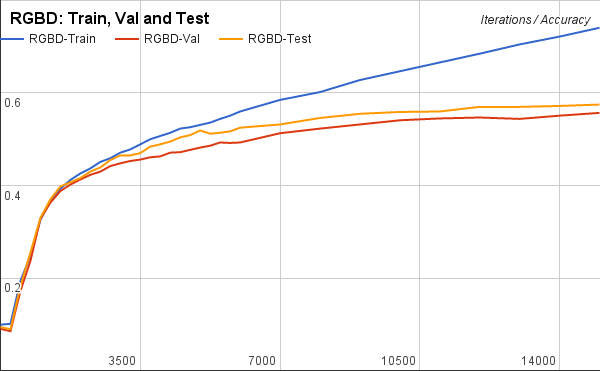
\includegraphics[width=\linewidth]{../presentation/rgbd_cnn.png}
	\caption{RGBD CNN Train/Val/Test Accuracy, Iterations}
	\label{fig:mixtest2}
\end{figure}
%-------------------------------------------------------------------------
\section{Further Work}
\subsection{Depth Estimation}
We\rq{}ve mentioned that depth estimation is an ill-posed problem, 
since we can not find the ground truth depth map which would allow us compare the performance of 
different depth estimation models.
However, using the accuracy metric we proposed, performance can be measured indirectly.
The only drawback is that our running on our metric need much more time than most other typical metrics.
If we had more time, we would measure the performance of existing depth estimation models.


\subsection{Learning on RGBD Dataset}
In our experiment, we didn\rq{}t implement state-of-the-art image classification model \cite{he2015deep} for simplicity.
We consider to test RGBD dataset on that model. 
Maybe we can witness accuracy surpassing current record.

We also plan to build more RGBD datasets and publish them for research usage.

\subsection{Learning on RGBD (ground-truth depth) vs RGBD (estimated depth)}
Compare the accuracy of Learning on RGBD (ground-truth) vs RGBD (estimated). It is possible that RGBD (estimated) can achieve better result than RGBD (groud-truth), since RGBD (estimated) are obtained by deep neural network which extract some high level features automatically. We need to further compare nd investigate learning of Learning on RGBD (ground-truth) vs RGBD (estimated).

%-------------------------------------------------------------------------
\section{Conclusion}
We successfully reimplemented the state-of-the-art depth-estimation model using
We create the first RGBD image dataset for CIFAR10, and investigate its quality 
using our metric.
We define a transfer learning accuracy metric for depth prediction problem.
On RGBD CIFAR, we prove that depth channel has a better feature representation.
We also show that training on RGBD images can somehow improve image 
classification accuracy.
	
	% use section* for acknowledgment
	\section*{Acknowledgment}
	
	
	The authors would like to thank Metehan Ozten.
	
	
	% Can use something like this to put references on a page
	% by themselves when using endfloat and the captionsoff option.
	\ifCLASSOPTIONcaptionsoff
	\newpage
	\fi
	
{\small
	\printbibliography
}
	
	% biography section
	% 
	% If you have an EPS/PDF photo (graphicx package needed) extra braces are
	% needed around the contents of the optional argument to biography to prevent
	% the LaTeX parser from getting confused when it sees the complicated
	% \includegraphics command within an optional argument. (You could create
	% your own custom macro containing the \includegraphics command to make things
	% simpler here.)
	%\begin{IEEEbiography}[{\includegraphics[width=1in,height=1.25in,clip,keepaspectratio]{mshell}}]{Michael Shell}
	% or if you just want to reserve a space for a photo:
	
	\begin{IEEEbiography}[{\includegraphics[width=1in,height=1.25in,clip,keepaspectratio]{me}}]{Yihui He}
		is doing the B.S. degree in computer science at Xi'an Jiaotong University.
		He is currently an intern at Megvii Technology Inc., Beijing. His research interests include Computer Vision, Computer Network, and Security Game.
	\end{IEEEbiography}

	
	% You can push biographies down or up by placing
	% a \vfill before or after them. The appropriate
	% use of \vfill depends on what kind of text is
	% on the last page and whether or not the columns
	% are being equalized.
	
	%\vfill
	
	% Can be used to pull up biographies so that the bottom of the last one
	% is flush with the other column.
	%\enlargethispage{-5in}
	
	
	
	% that's all folks
\end{document}


